
\section{Computer architecture}
It mainly consists of the following elements:
\begin{itemize}
    \item Central Processing Unit (CPU)
    \item Memory Unit
    \item Input/Output Devices( Mass Storage Unit, Keyboard, Display\ldots)
\end{itemize}

Furthermore, the CPU itself consists of three main components:
\begin{itemize}
    \item Control Unit (CU)
    \item Arithmetic/Logic Unit (ALU)
    \item Registers
\end{itemize}

\subsection{Memory}

A computer's memory is where the temporary data and instructions of currently
running programs are located. A computer's memory is also known as Primary
Memory. It is the primary location the CPU uses to retrieve and process data.
It does so very frequently, so the memory must be extremely fast in storing and
retrieving data and instructions.

There are two main types of memory:

\subsubsection{Cache}

memory is usually located within the CPU itself. It runs at the same clock speed as the CPU. 

There are usually three levels of cache memory, depending on their closeness to the CPU core:

\begin{itemize}
        \item Level 1 Cache Usually in kilobytes, the fastest memory
            available, located in each CPU core
        \item Level 2 Cache Usually in megabytes, shared between all CPU cores.
        \item Level 3 Cache Usually in megabytes (Not all CPUs use L3.)
\end{itemize}

\subsubsection{ RAM} located far away from the CPU cores  is much slower than cache
memory. Accessing data from RAM addresses takes many more instructions.

For example, retrieving an instruction from the registers takes only one clock
cycle, and retrieving it from the L1 cache takes a few cycles, while retrieving
it from RAM takes around 200 cyclesa.

In the past, with 32-bit addresses, memory addresses were limited from
0x00000000 to 0xffffffff. This meant that the maximum possible RAM size was 232
bytes, which is only 4 gigabytes, at which point we run out of unique
addresses. With 64-bit addresses, the range is now up to 0xffffffffffffffff,
with a theoretical maximum RAM size of 264 bytes, which is around 18.5 exabytes
(18.5 million terabytes), so we shouldn't be running out of memory addresses
anytime soon.

When a program is run, all of its data and instructions are moved from the
storage unit to the RAM to be accessed when needed by the CPU. 
When a program is closed, its data is removed or made available to re-use from
the RAM.


\subsubsection{Memory Layout of a program}
 The actual layout of a program's in-memory image is left entirely up to the
 operating system, and often the program itself as well. This article focus on
 the concepts of code and data segments of a program and does not take any
 specific platform into account. For a running program both the machine
 instructions (program code) and data are stored in the same memory space. The
 memory is logically divided into text and data segments. Modern systems use a
 single text segment to store program instructions, but more than one segment
 for data, depending upon the storage class of the data being stored there.

 \begin{figure}
  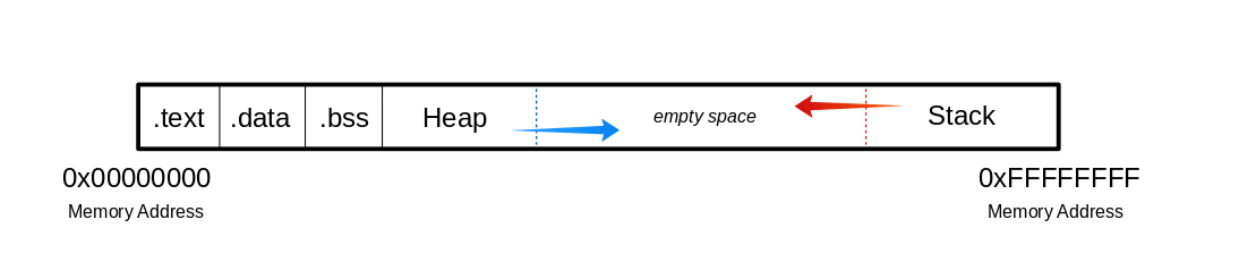
\includegraphics[width=\linewidth]{binary/intro/images/memory-layout.png}
  \caption{Linux memory layout}
  \label{fig:linux-memory-layout}
\end{figure}

{\bf Text Segment}

text segment contains machine code of the compiled
program. The text segment of an executable object file is often read-only
segment that prevents a program from being accidentally modified.

{\bf Data Segments}

Data segment stores program data. This data could be in form of initialized or
uninitialized variables, and it could be local or global. Data segment is
further divided into four sub-data segments (initialized data segment,
uninitialized or \verb+.bss+ data segment, stack, and heap) to store variables
depending upon if they are local or global, and initialized or uninitialized.

{\bf Initialized Data or Data Segment}

Initialized data or simply data segment stores all global, static, constant,
and external variables (declared with \verb+extern+ keyword) that are initialized
beforehand.


{\bf Uninitialized Data or bss Segment}

Contrary to initialized data segment, uninitialized data or \verb+.bss+ segment stores
all uninitialized global, static, and external variables.This section occupies
no actual space in the object file; it is merely a place holder. Object file
formats distinguish between initialized and uninitialized variables for space
efficiency; uninitialized variables do not have to occupy any actual disk space
in the object file.

{\bf Stack Segment}

Stack segment is used to store all local variables and is used for passing
arguments to the functions along with the return address of the instruction
which is to be executed after the function call is over. Local variables have a
scope to the block which they are defined in; they are created when control
enters into the block. Local variables do not appear in data or bss segment.
Also all recursive function calls are added to stack. Data is added or removed
in a last-in-first-out manner to stack. When a new stack frame needs to be
added (as a result of a newly called function), the stack grows downward.

{\bf Heap Segment}
 Heap segment is also part of RAM where dynamically allocated variables are
 stored. 

The stack and heap are traditionally located at opposite ends of the process's
virtual address space.

\subsection{IO/Storage}

Finally, we have the Input/Output devices, like the keyboard, the screen, or
the long-term storage unit, also known as Secondary Memory. The processor can
access and control IO devices using Bus Interfaces, which act as 'highways' to
transfer data and addresses, using electrical charges for binary data.

Each Bus has a capacity of bits it can carry simultaneously. This usually is a multiple of 4-bits, ranging up to 128-bits. Bus interfaces are also usually used to access memory and other components outside the CPU itself. 

Unlike primary memory the storage unit stores permanent data.

The storage unit is the slowest to access. 
